\chapter{Implementacija i korisničko sučelje}
		
		
		\section{Korištene tehnologije i alati}
		
			%\textbf{\textit{dio 2. revizije}}
			
			 %\textit{Detaljno navesti sve tehnologije i alate koji su primijenjeni pri izradi dokumentacije i aplikacije. Ukratko ih opisati, te navesti njihovo značenje i mjesto primjene. Za svaki navedeni alat i tehnologiju je potrebno \textbf{navesti internet poveznicu} gdje se mogu preuzeti ili više saznati o njima}.
			
			Komunikacija među članovima tima odvijala se putem aplikacije \underline{WhatsApp}\footnote[1]{\href{https://web.whatsapp.com/}{https://web.whatsapp.com/}}. Za izradu UML dijagrama korišten je alat \underline{Astah Professional}\footnote[2]{\href{https://astah.net/products/astah-uml/}{https://astah.net/products/astah-uml/}}. Za upravljanje izvornim kodom korišten je \underline{Git}\footnote[3]{\href{https://git-scm.com/}{https://git-scm.com/}}, a kao udaljeni repozitorij projekta git platforma \underline{GitHub}\footnote[4]{\href{https://github.com/}{https://github.com/}}.\\
			Kao razvojno okruženje korišten je \underline{Microsoft Visual Studio}\footnote[5]{\href{https://visualstudio.microsoft.com/}{https://visualstudio.microsoft.com/}}, koji pruža različite alate za razvoj računalnih programa kao što su web stranice, web usluge i mobilne aplikacije.\\
			Za izradu backenda aplikacije korišten je radni okvir \underline{.NET Framework}\footnote[6]{\href{https://dotnet.microsoft.com/en-us/}{https://dotnet.microsoft.com/en-us/}} i jezik \underline{C\#}\footnote[7]{\href{https://learn.microsoft.com/en-us/dotnet/csharp/}{https://learn.microsoft.com/en-us/dotnet/csharp/}}, a za izradu frontenda \underline{React}\footnote[8]{\href{https://react.dev/}{https://react.dev/}} i jezik \underline{JavaScript}\footnote[9]{\href{https://www.javascript.com/}{https://www.javascript.com/}}. .NET Framework je razvojni okvir tvrtke Microsoft koji omogućava razvoj, implementaciju i pokretanje web aplikacija. Pri razvoju aplikacija nudi gotova rješenja i funkcionalnosti kako bi se ubrzao i pojednostavio proces razvoja aplikacije. React je knjižnica pisana u JavaScriptu, a koristi se za izgradnju korisničkih sučelja ili njegovih dijelova.
			
			\eject 
		
	
		\section{Ispitivanje programskog rješenja}
			
			%\textbf{\textit{dio 2. revizije}}\\
			
			 %\textit{U ovom poglavlju je potrebno opisati provedbu ispitivanja implementiranih funkcionalnosti na razini komponenti i na razini cijelog sustava s prikazom odabranih ispitnih slučajeva. Studenti trebaju ispitati temeljnu funkcionalnost i rubne uvjete.}
			 
			 Ispitivanje je aktivnost s ciljem poboljšanja kvalitete proizvoda tako da se pronalaze i otklanjaju greške u implementaciji. Glavni pojam u ispitivanju je ispitni slučaj koji se definira kao uređeni par ulaznog podatka i očekivanog izlaznog podatka, koji je zabilježen prije provođenja ispitivanja.
	
			
			\subsection{Ispitivanje komponenti}
			%\textit{Potrebno je provesti ispitivanje jedinica (engl. unit testing) nad razredima koji implementiraju temeljne funkcionalnosti. Razraditi \textbf{minimalno 6 ispitnih slučajeva} u kojima će se ispitati redovni slučajevi, rubni uvjeti te izazivanje pogreške (engl. exception throwing). Poželjno je stvoriti i ispitni slučaj koji koristi funkcionalnosti koje nisu implementirane. Potrebno je priložiti izvorni kôd svih ispitnih slučajeva te prikaz rezultata izvođenja ispita u razvojnom okruženju (prolaz/pad ispita). }
			
			Ispitivanje jedinica podrazumijeva ispitivanje funkcionalnosti najmanjih dijelova programa kao što su razredi, pripadajuće metode i atributi.
			
			
			
			\subsection{Ispitivanje sustava}
			
			 \textit{Potrebno je provesti i opisati ispitivanje sustava koristeći radni okvir Selenium\footnote{\url{https://www.seleniumhq.org/}}. Razraditi \textbf{minimalno 4 ispitna slučaja} u kojima će se ispitati redovni slučajevi, rubni uvjeti te poziv funkcionalnosti koja nije implementirana/izaziva pogrešku kako bi se vidjelo na koji način sustav reagira kada nešto nije u potpunosti ostvareno. Ispitni slučaj se treba sastojati od ulaza (npr. korisničko ime i lozinka), očekivanog izlaza ili rezultata, koraka ispitivanja i dobivenog izlaza ili rezultata.\\ }
			 
			 \textit{Izradu ispitnih slučajeva pomoću radnog okvira Selenium moguće je provesti pomoću jednog od sljedeća dva alata:}
			 \begin{itemize}
			 	\item \textit{dodatak za preglednik \textbf{Selenium IDE} - snimanje korisnikovih akcija radi automatskog ponavljanja ispita	}
			 	\item \textit{\textbf{Selenium WebDriver} - podrška za pisanje ispita u jezicima Java, C\#, PHP koristeći posebno programsko sučelje.}
			 \end{itemize}
		 	\textit{Detalji o korištenju alata Selenium bit će prikazani na posebnom predavanju tijekom semestra.}
			
			\eject 
		
		
		\section{Dijagram razmještaja}
			
			%\textbf{\textit{dio 2. revizije}}
			
			 %\textit{Potrebno je umetnuti \textbf{specifikacijski} dijagram razmještaja i opisati ga. Moguće je umjesto specifikacijskog dijagrama razmještaja umetnuti dijagram razmještaja instanci, pod uvjetom da taj dijagram bolje opisuje neki važniji dio sustava.}
			
			Na poslužiteljskom računalu smješteni su web poslužitelj i poslužitelj baze podataka. Klijenti pristupaju web aplikaciji putem web preglednika. Sustav je temeljen na arhitekturi "klijent-poslužitelj", a komunikacija između računala korisnika i poslužitelja odvija se putem HTTP veze.
			
			\begin{figure}[H]
				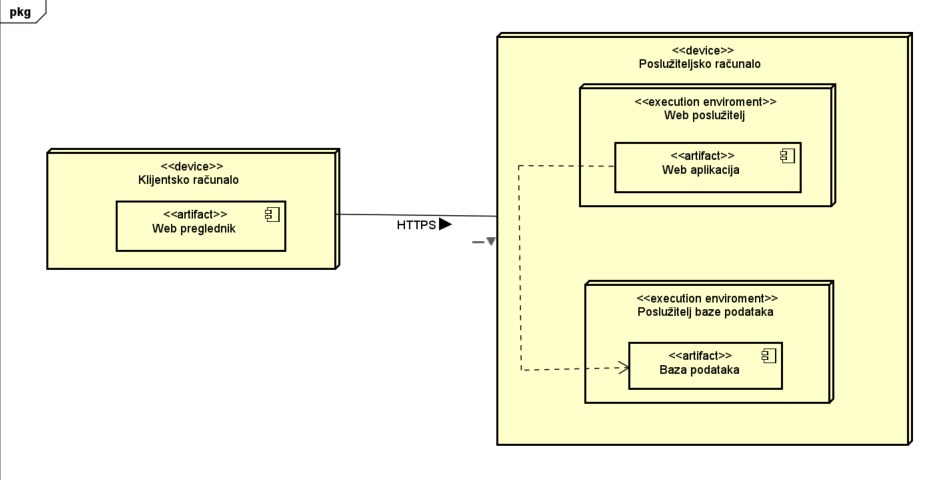
\includegraphics[width=\textwidth]{dijagram_razmjestaja.JPEG}
				\centering
				\caption{Dijagram razmještaja}
				\label{fig:dijagramrazmjestaja}
			\end{figure}
			
			\eject 
		
		\section{Upute za puštanje u pogon}
		
			\textbf{\textit{dio 2. revizije}}\\
		
			 \textit{U ovom poglavlju potrebno je dati upute za puštanje u pogon (engl. deployment) ostvarene aplikacije. Na primjer, za web aplikacije, opisati postupak kojim se od izvornog kôda dolazi do potpuno postavljene baze podataka i poslužitelja koji odgovara na upite korisnika. Za mobilnu aplikaciju, postupak kojim se aplikacija izgradi, te postavi na neku od trgovina. Za stolnu (engl. desktop) aplikaciju, postupak kojim se aplikacija instalira na računalo. Ukoliko mobilne i stolne aplikacije komuniciraju s poslužiteljem i/ili bazom podataka, opisati i postupak njihovog postavljanja. Pri izradi uputa preporučuje se \textbf{naglasiti korake instalacije uporabom natuknica} te koristiti što je više moguće \textbf{slike ekrana} (engl. screenshots) kako bi upute bile jasne i jednostavne za slijediti.}
			
			
			 \textit{Dovršenu aplikaciju potrebno je pokrenuti na javno dostupnom poslužitelju. Studentima se preporuča korištenje neke od sljedećih besplatnih usluga: \href{https://aws.amazon.com/}{Amazon AWS}, \href{https://azure.microsoft.com/en-us/}{Microsoft Azure} ili \href{https://www.heroku.com/}{Heroku}. Mobilne aplikacije trebaju biti objavljene na F-Droid, Google Play ili Amazon App trgovini.}
			
			
			\eject 